\documentclass[20pt,margin=5mm, innermargin=6mm, blockverticalspace=6mm, colspace=6mm]{tikzposter}
\usepackage[utf8]{inputenc}
\geometry{paperwidth=42.0cm,paperheight=59.4cm}
% \usetheme{Simple}
% \usecolorstyle{Spain}
% \usebackgroundstyle{Empty}
% \usetitlestyle{Filled}
% \useblockstyle{Basic}
\tikzposterlatexaffectionproofoff
\usepackage{amsmath}
\usepackage{enumitem}


\useblockstyle[titleinnersep=4mm, bodyinnersep = 6mm]{Slide}
\renewcommand*\familydefault{cabin}
\usepackage[sfdefault,condensed]{cabin}
\usepackage[T1]{fontenc}
\usepackage{fix-cm}
\usepackage{tikz,multicol}
\usepackage{capt-of}
\usepackage{titlesec}

\definecolor{greenone}{RGB}{21,75,52}
\definecolor{greentwo}{RGB}{25,97,66}
\definecolor{greenthree}{RGB}{16,57,39}
\definecolor{mygray}{RGB}{203,203,203}
\definecolorstyle{myColorStyle} {
    \colorlet{colorOne}{greenone}
    \colorlet{colorTwo}{greentwo}
    \colorlet{colorThree}{greenthree}
    \colorlet{colorFour}{mygray}
    }{
    % Background Colors
    \colorlet{backgroundcolor}{colorOne}
    \colorlet{framecolor}{colorOne}
    % Title Colors
    \colorlet{titlefgcolor}{white}
    \colorlet{titlebgcolor}{colorTwo}
    % Block Colors
    \colorlet{blocktitlebgcolor}{colorFour}
    \colorlet{blocktitlefgcolor}{colorTwo}
    \colorlet{blockbodybgcolor}{white}
    \colorlet{blockbodyfgcolor}{black}
    % Innerblock Colors
    \colorlet{innerblocktitlebgcolor}{white}
    \colorlet{innerblocktitlefgcolor}{black}
    \colorlet{innerblockbodybgcolor}{white}
    \colorlet{innerblockbodyfgcolor}{black}
    % Note colors
    \colorlet{notefgcolor}{black}
    \colorlet{notebgcolor}{white}
    \colorlet{notefrcolor}{white}
}

\usecolorstyle{myColorStyle}

\usebackgroundstyle{Rays}
\usepackage{adjustbox}
\usetitlestyle{Empty}

\makeatletter %To make columns scale to custom width 
\setlength{\TP@visibletextwidth}{\textwidth-2\TP@innermargin}
\setlength{\TP@visibletextheight}{\textheight-2\TP@innermargin}
\makeatother

\titlespacing*{\subsection}{0pt}{10pt}{0pt}

%shifts bullets to left margin for all document
%\setitemize{itemsep=10pt,topsep=0pt,parsep=0pt,partopsep=0pt, leftmargin= 20pt}

%only for a list
%\begin{itemize}[noitemsep,topsep=0pt,parsep=0pt,partopsep=0pt]
 
%\graphicspath{{images/}}

%%%%%%%%%%%%%%%%%%%%%%%%%%%%%%%%%%%%%%%%%%%%%%%%%%%%%%%%%%%%%%%%%%%%%%%%

\title{\parbox{\linewidth}{\vspace{-4.0cm} \centering \semiHUGE Temporal turnover of plant-pollinator interaction networks}}
\author{\vspace{-80pt} % space between title and author
  {\begin{minipage}{7.5cm}
    \hfill
    \vspace{-20pt}
    \flushleft
    
\includegraphics[trim=0cm 8cm 0cm 8cm,clip,width=7.5cm]{Imperial_Whitelogo.pdf}
  \end{minipage}
    \vspace{-20pt}
    \hspace{2pt}}
  {\begin{minipage}{22cm}
    \centering
        { \Large Jia Le, Lim \\
        \vspace{2pt}
        \normalsize jialelim@hotmail.com \\
         \vspace{-28pt}
          \normalsize Department of Life Sciences, Silwood Park Campus, Imperial College London}
  \end{minipage}
    \vspace{-20pt}
  \hspace{2pt}}
  {\begin{minipage}{8cm}
    \hfill
    \flushright
    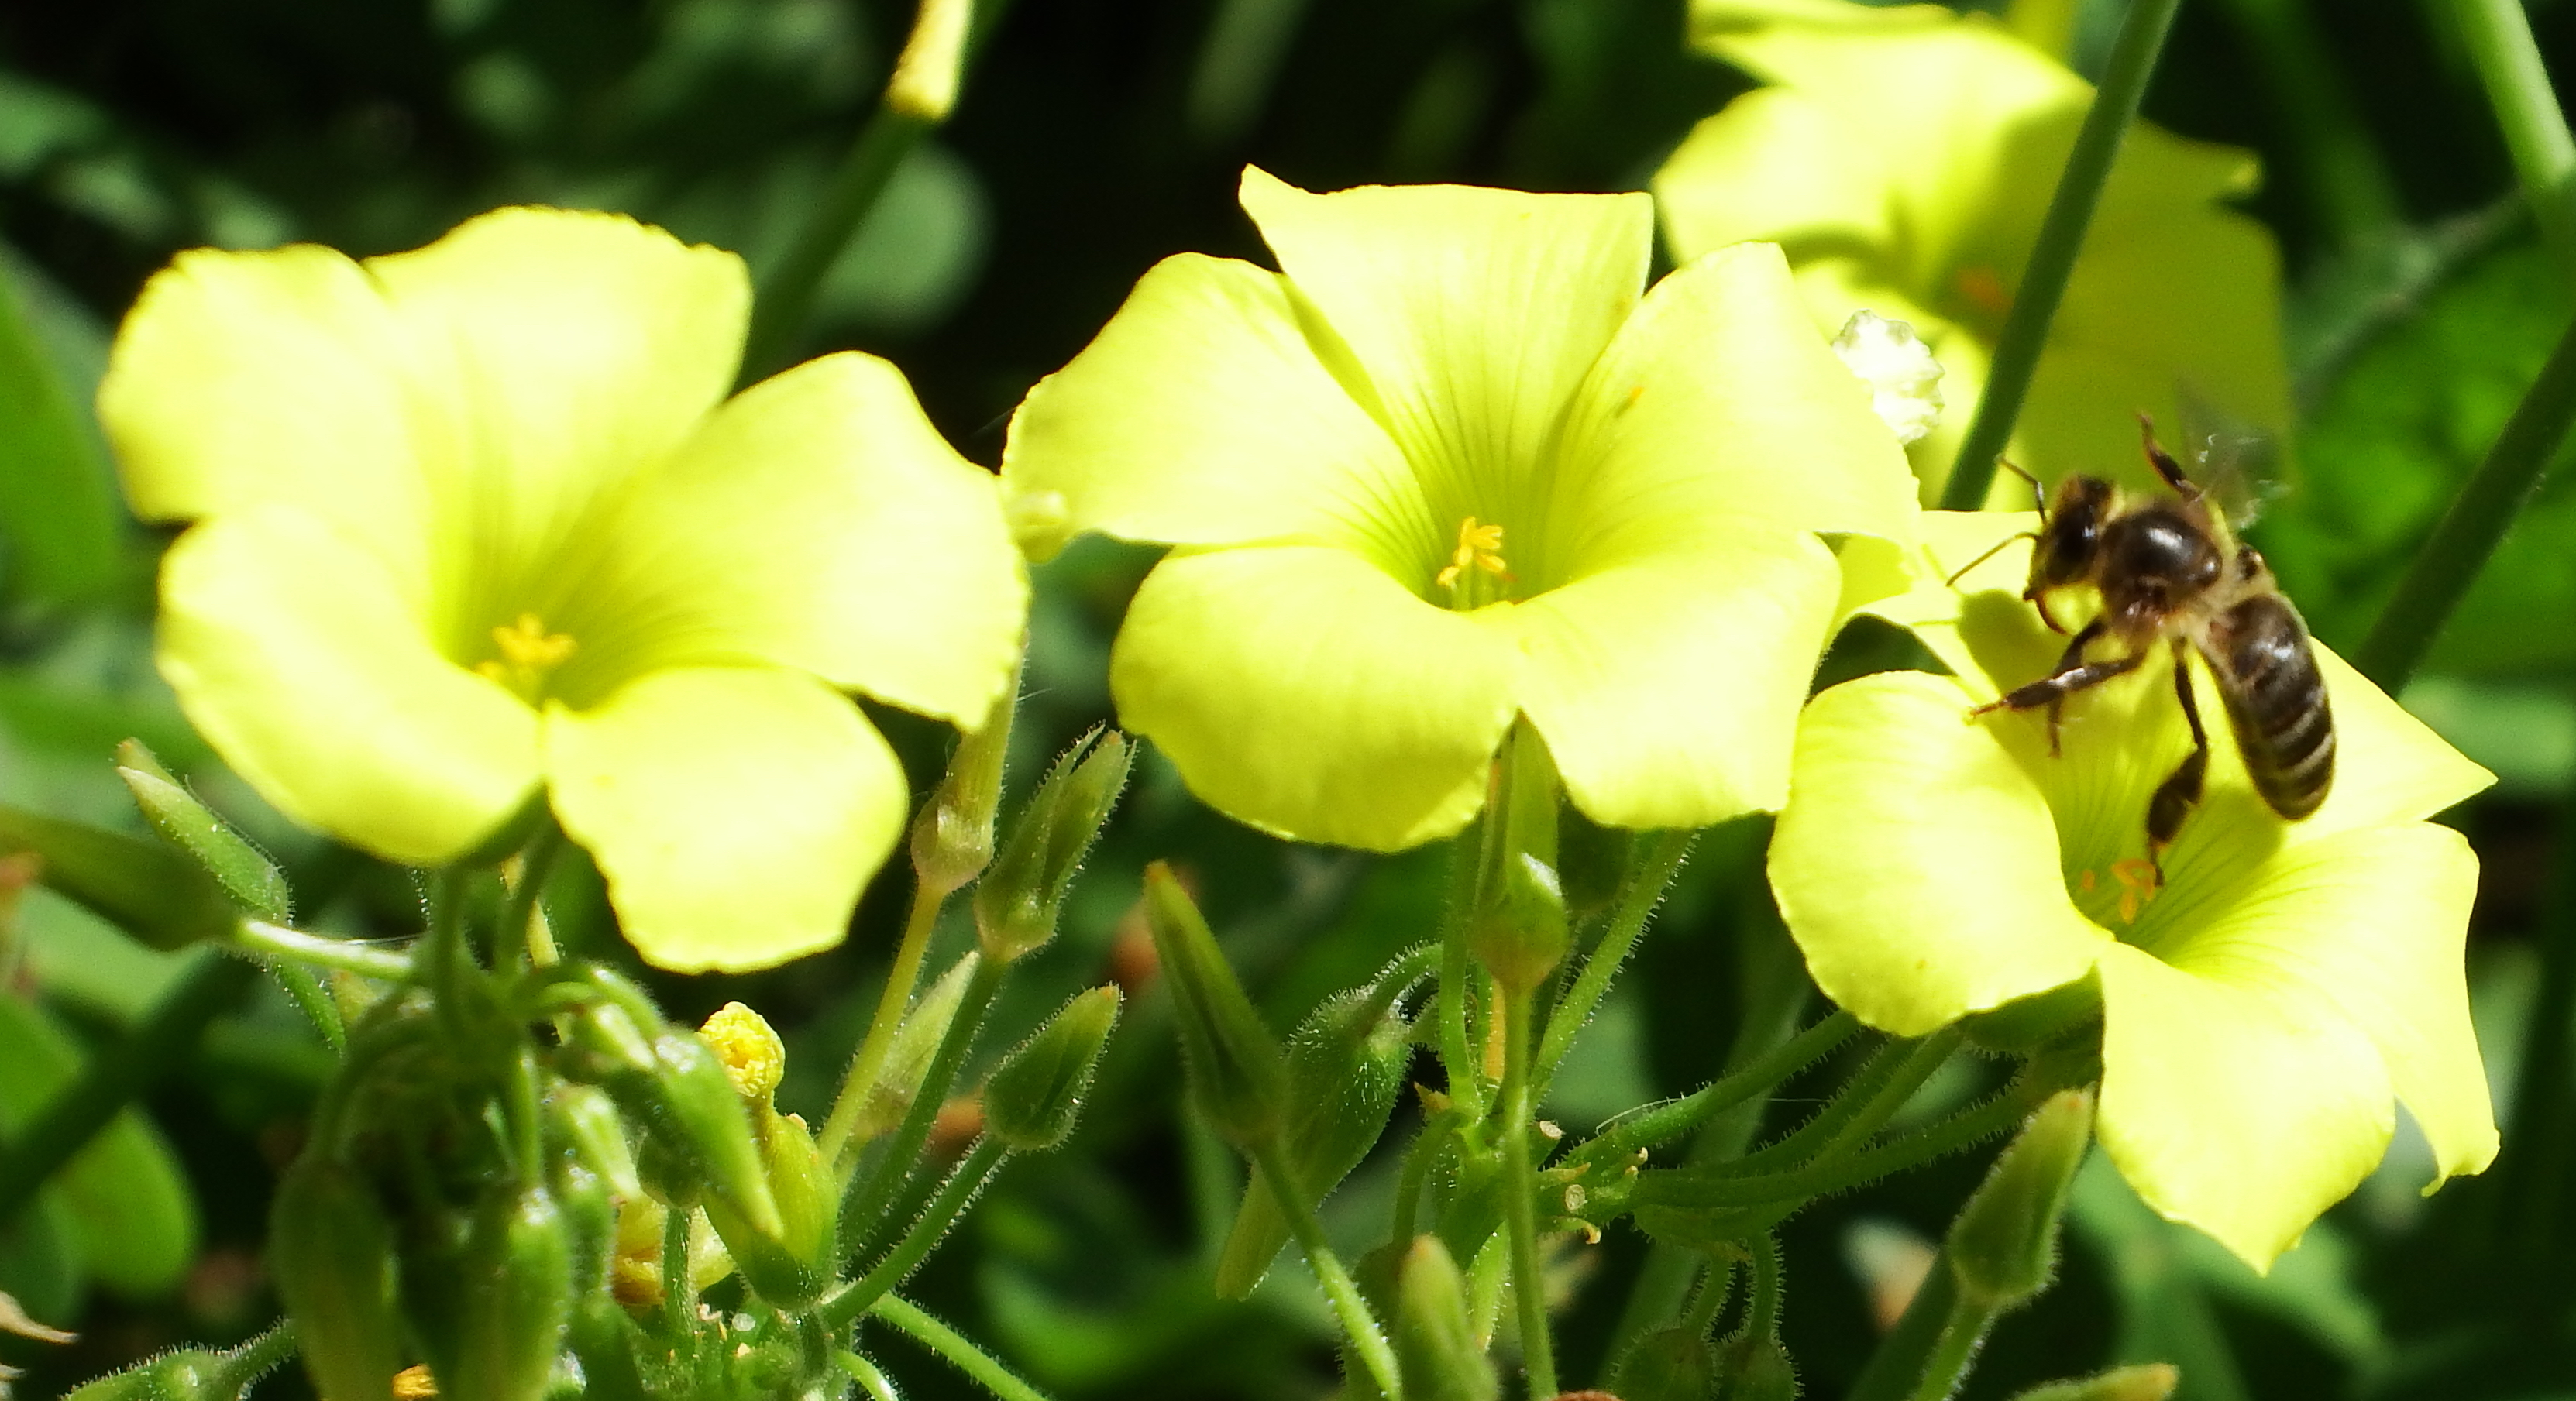
\includegraphics[trim=0cm 4cm 0cm 4cm,clip,width=7.5cm]{picture.JPG}
  \end{minipage}
  \vspace{-20pt}}
  }

%%%%%%%%%%%%%%%%%%%%%%%%%%%%%%%%%%%%%%%%%%%%%%%%%%%%%%%%%%%%%%%%%%%%%%%%
\makeatletter
\newcommand\semiHUGE{\@setfontsize\semiHUGE{40}{27.38}}
\makeatother

\begin{document}
\node[xshift=-20cm, at=(topright),opacity=0.8]{\includegraphics[width=\paperwidth, height=12cm]{head1low.jpg}} ;

\maketitle[titletoblockverticalspace=5mm]

  %%%%%%%%%%%%%%%%%%%%%%%%%%%%%%%%%%%%%%%%%%%%%%%%%%%%%%%%%%%%%%%%%%%%%%%%
%Introduction in form of a question?
\block{\Large \hspace{0.5pt} Dynamics of bee-flower interactions}{

  \normalsize
     %Brief Introduction explaining broader significance of research problem and the gap in knowledge that is being addressed
     %%% Bee-flower interactions differ drastically between subsequent seasons or even weeks. However, this high interaction turnover has been largely overlooked by previous studies, which assume a static picture of pollination networks. Understanding how and why bee-flower interactions vary over time is crucial in the conservation of bees, and in the continuation of their pollination services. Moreover, climate change can result in fluctuating flowering times, thereafter indirectly sabotaging bee-flower interactions. \\
     Understanding how and why plant-pollinator networks (e.g., bee-flower) interactions vary over time is crucial in the conservation of pollinators, and in the continuation of their pollination services. Moreover, climate change can result in fluctuating flowering times, therefore affecting or driving turnover in plant-pollinator interactions. The structure of bee-flower interaction networks are likely to differ between seasons or even shorter timescales of weeks to months. However, this interaction turnover has been largely been ignored by previous research on plant-pollinator networks, which assume a static picture of pollination networks. \\
  
  \begin{minipage}[]{0.57\linewidth}
    \vspace{-13pt}
    \subsection*{I ask...}
     %research plan
    \begin{itemize}[itemsep=5pt,topsep=0pt,parsep=0pt,partopsep=0pt, leftmargin=20pt]
    \item Does temperature, precipitation or humidity affect bee-flower interaction turnover?
    \item Does bee-flower interaction turnover differ between seasons?
    \item Does bee-flower interaction turnover of the tropics differ from those of the temperate regions?
    \end{itemize}

  \end{minipage}   
  \hspace{.8cm}    
  \begin{minipage}[]{0.40\linewidth}
     \vspace{-15pt}
   \subsection*{Data}
   %Materials and methods
    \begin{itemize}[itemsep=5pt,topsep=0pt,parsep=0pt,partopsep=0pt, leftmargin=20pt]
    \item \textit {Species level:} More than 200 different species of plants and bees
    \item \textit{Interactions level:} More than 600 unique interactions and more than 3500 recorded interactions across 39 months
    \end {itemize}
    \end{minipage}

    \subsection*{\centering Aim: \normalfont To investigate the effect of climate on bee-flower interaction turnover.} 
   %A clear statement of the project aim or aims
 }

 %%%%%%%%%%%%%%%%%%%%%%%%%%%%%%%%%%%%%%%%%%%%%%%%%%%%%%%%%%%%%%%%%%%%%%%%


%%%%%%%%%%%%%%%%%%%%%%%%%%%%%%%%%%%%%%%%%%%%%%%%%%%%%%%%%%%%%%%%%%%%%%%%%%%%%%%%%%%%%%%%%%%%%%%%%%%%%%%%%%%%%%%%%%
\begin{columns}
\column{0.25}
  \block{\Large \hspace{3pt}Calculating turnover}{
    \normalsize
    \vspace{20pt}
Whittaker's dissimilarity index, $\boldsymbol{ \beta_{int}}$, reflects the difference between two successive monthly networks.
	\vspace{0pt} \\
	
    \begin{align*}
      \boldsymbol{ \beta_{int}} & = \frac{a + b + c}{(2a + b + c)/2} - 1
    \end{align*}\\

    \vspace{0pt}
    where:    
    \begin{itemize}
     \item $a$ is the number of interactions shared between the two networks  
    \item $b$ and $c$ are the number of unique interactions in the two networks
    \end{itemize}
 \vspace{20pt}
 $\boldsymbol{ \beta_{int}}$ ranges from 0 to 1. \\
 A higher $\boldsymbol{ \beta_{int}}$ reflects a higher difference between monthly networks.


  }

\column{0.75}
  \block{\Large \hspace{17pt} Preliminary Results}{ 
  \vspace{-30pt}
    \flushright
    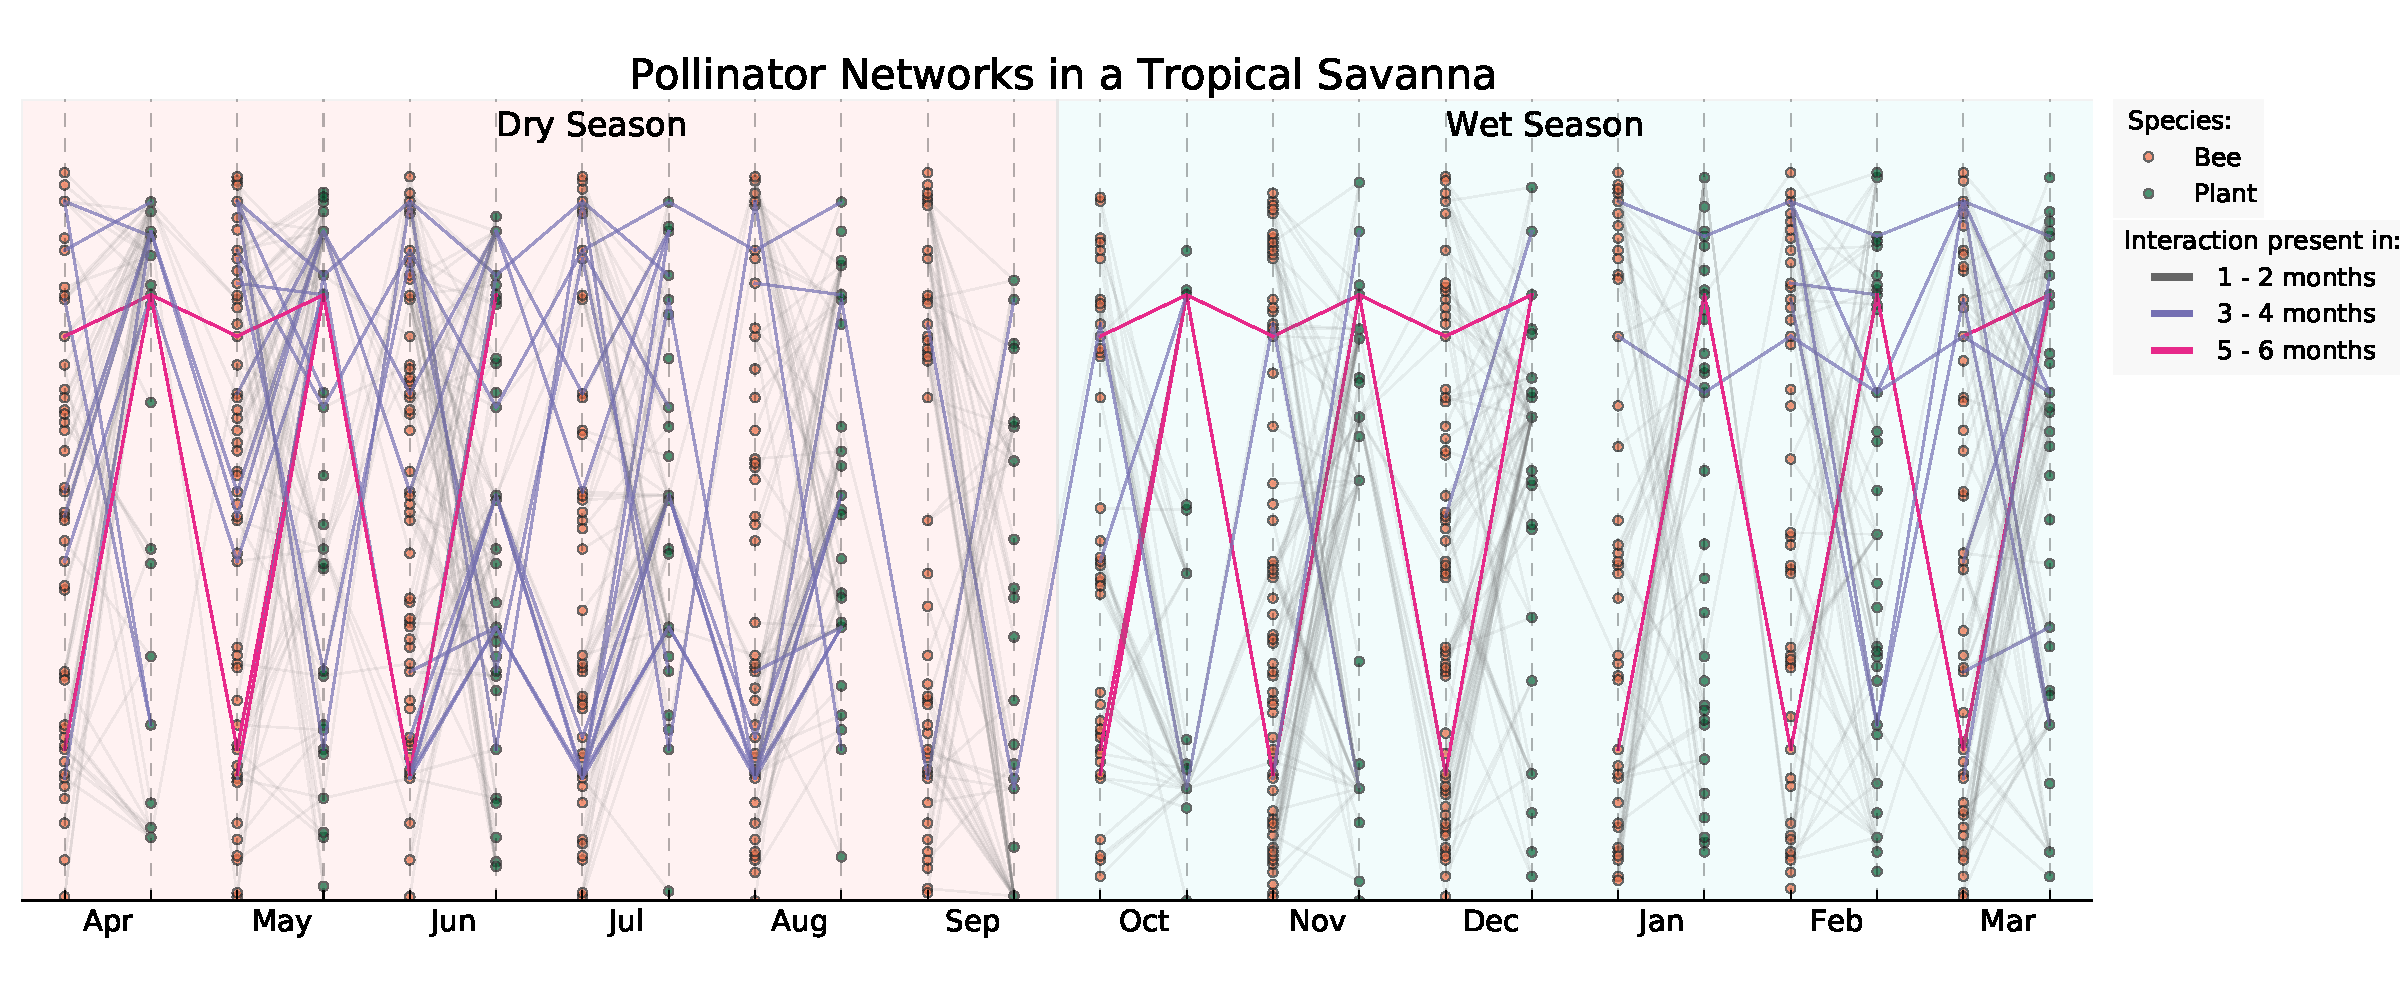
\includegraphics[width=\linewidth]{network4.pdf} 
     \vspace{-50pt}
\flushleft \footnotesize Figure 1: Monthly bee pollinator networks from April 1995 to Mar 1996. \\
 Average monthly precipitation sum = 22.84 mm(Dry Season), 239.6mm (Wet Season) \\
 \vspace{-155pt}
    \centering
    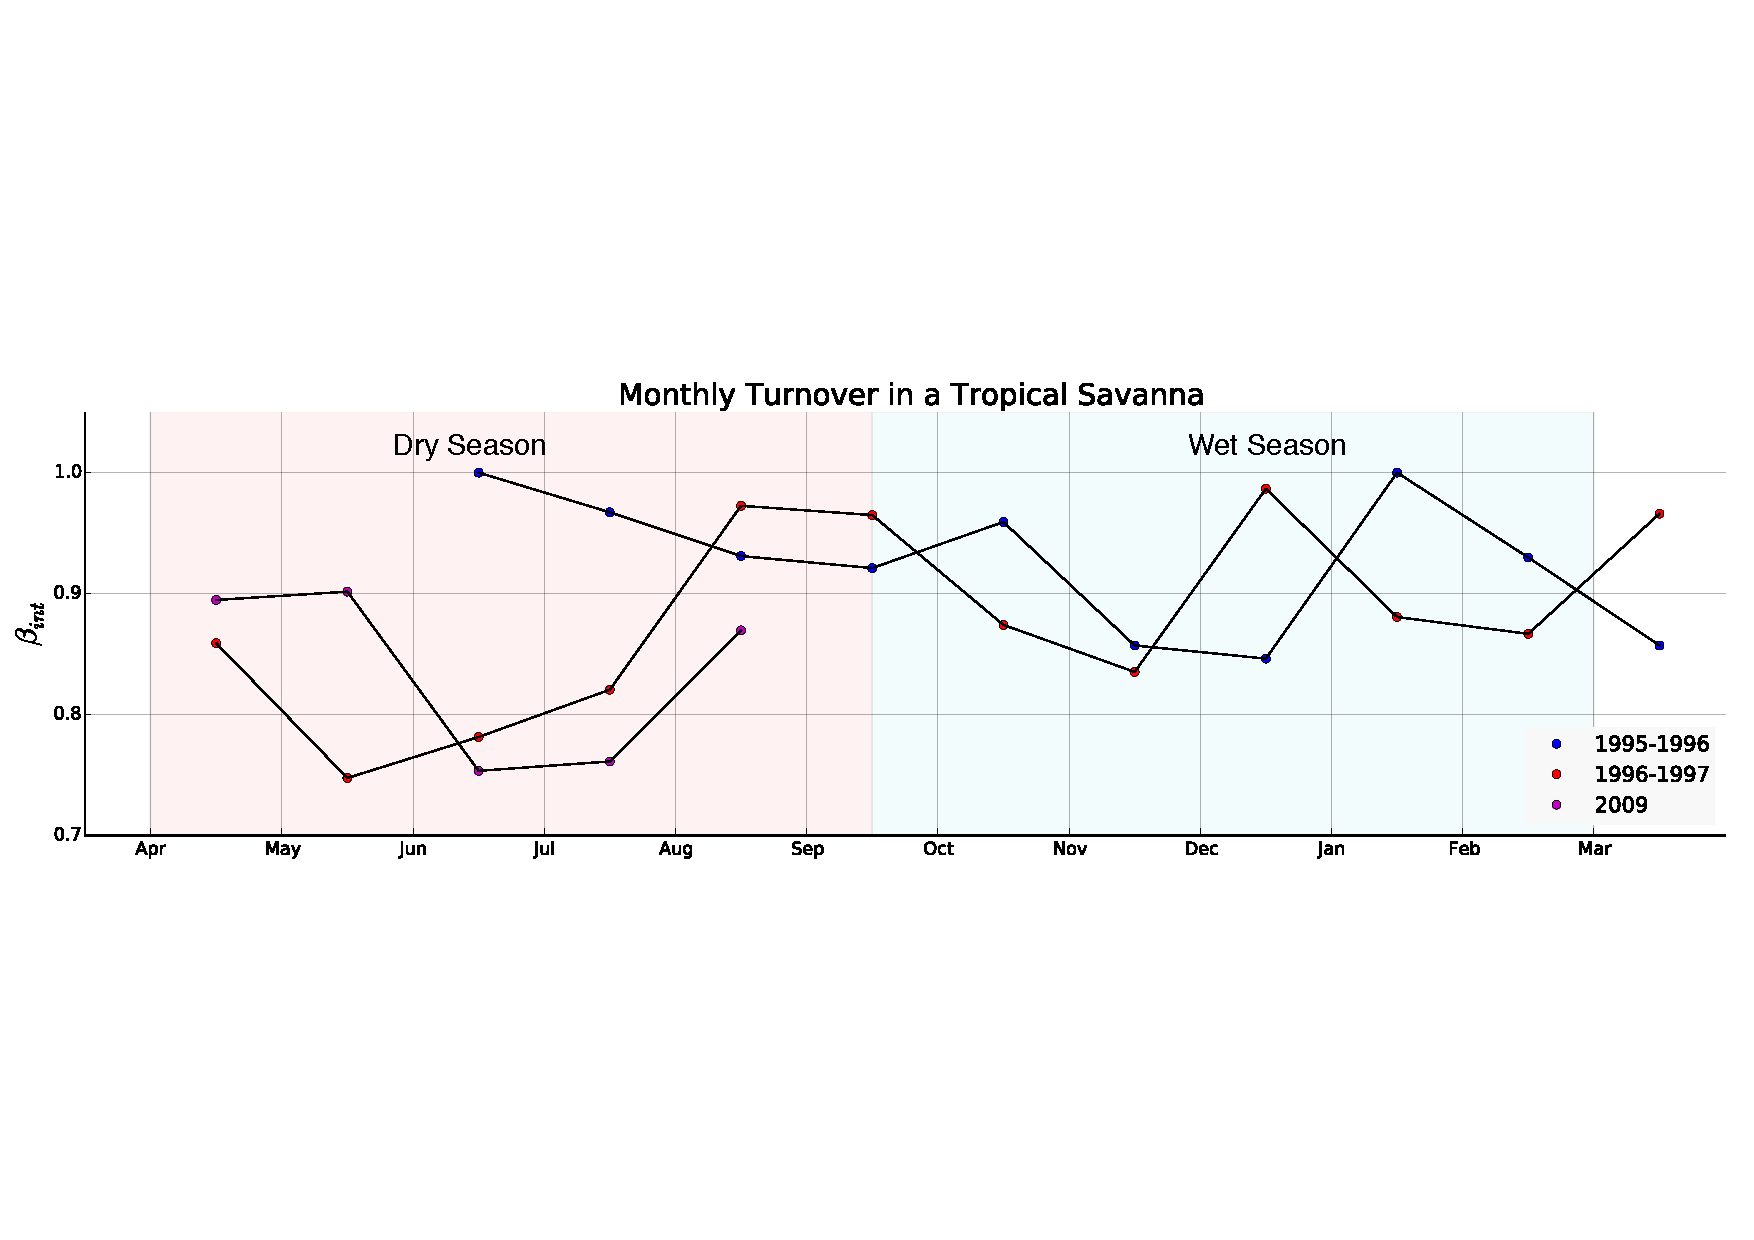
\includegraphics[width=\linewidth]{turnover.pdf}
    \footnotesize 
   \vspace{-185pt}
    %If you include your own results (nice if available but not necessary given the early stage of the project) make sure data clearly explained
    
  }

\end{columns}

%%%%%%%%%%%%%%%%%%%%%%%%%%%%%%%%%%%%%%%%%%%%%%%%%%%%%%%%%%%%%%%%%%%%%%%%
\begin{columns}


  \column{0.6}
  \block{\Large \hspace{17pt}Conclusions and Ongoing work}{ 
  \normalsize	

    \begin{itemize}[itemsep=5pt,topsep=0pt,parsep=0pt,partopsep=0pt, leftmargin=*]
    \item Monthly bee-flower interaction turnover is higher than ever reported before. Mean turnover rate is 
    \item There are no significant differences between turnover rates within seasons and between seasons.
    \item There is a periodic pattern in turnover of bee-flower interactions.
    \item Currently determining if precipitation and temperature are strong drivers of bee-flower interaction turnover.
    \end{itemize}      
%Conclusions that can be drawn and future directions
}
  %%%%%%%%%%%%%%%%%%%%%%%%%%%%%%%%%%%%%%%%%%%%%%%%%%%%%%%%%%%%%%%%%%%%%%%%
  \column{0.4}
  \block{\Large \hspace{17pt}Possible challenges}{
    \normalsize
    \begin{itemize}[itemsep=5pt,topsep=0pt,parsep=0pt,partopsep=0pt, leftmargin=*]
    \item Insufficient data; However, $\boldsymbol{\beta_{int}}$ is rarely affected by small sample sizes.
    \item If climate does not affect bee-flower interaction turnover, other factors to be considered include bee body size and lifespan.
    \end{itemize}    
    %Discussion of research strategy (identification of potential problems and how these will be overcome)
}
  
\end{columns}

%%%%%%%%%%%%%%%%%%%%%%%%%%%%%%%%%%%%%%%%%%%%%%%%%%%%%%%%%%%%%%%%%%%%%%%%%%%%%%%%%%%%%%%%%%%%%%%%%%%%%%%%%%%%%%%%%%

\block[bodyverticalshift=2mm]{}{
\vspace{-10pt}
  \footnotesize 
  References:  
  \begin{itemize}[itemsep=0pt,topsep=0pt,parsep=0pt,partopsep=0pt, leftmargin=*]
  \item CaraDonna, P. J., Petry, W. K., Brennan, R. M., et. al. (2017). Interaction rewiring and the rapid turnover of plant-pollinator networks. \textit{Ecol. Letters}, 20: 385-394. doi:10.1111/ele.12740
  \item Simone, C.R., Simpson, B., Tidon, R., Neff, J., Pawar, S. (2015). Aseasonal pollinators connect seasonal modules in pollination networks from the Cerrado, a highly diverse seasonally dry neotropical savanna. [Not published]  
  \item Poisot, T., Canard, E., Mouillot, D., Mouquet, N. \& Gravel, D. (2012). The dissimilarity of species interaction networks. \textit{Ecol. Letters}, 11, 564-575

  \end{itemize}
  \vspace{5pt}
  \textit{Acknowledgements: Special thanks to M.C. BoaVentura and S. C. Cappellari for making their data set available for the analyses, as well as Samraat Pawar for his supervision and advice throughout this project.}
}


\end{document}
